\section{Important notes}

\frame{\tableofcontents[currentsection]}


\begin{frame}
    \frametitle{Blocking init with module supervisors}
    imagine the following supervision tree (note the PIDs)
    \vfill
    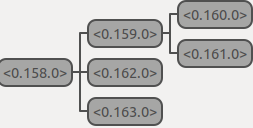
\includegraphics[scale=0.7]{12_simple_supervision_tree.png}
\end{frame}

\begin{frame}
    \frametitle{Code representation}
    \code[language=elixir,font=\scriptsize]{demo-code/04_note_root_sup.ex}
    \code[language=elixir,font=\scriptsize]{demo-code/05_note_sub_sup.ex}
\end{frame}

\begin{frame}
    \frametitle{Blocking init with module supervisors}
    \begin{itemize}
        \item Children are started sequentially
        \item Sub-supervisors their init only returns after starting childs!
    \end{itemize}
\end{frame}

\begin{frame}
    \frametitle{Child creation}
    \begin{center}
        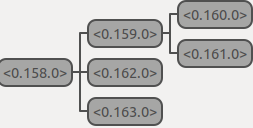
\includegraphics[scale=0.5]{12_simple_supervision_tree.png}
        \begin{itemize}
            \item Root supervisor -$>$ start child supervisor [WAIT FOR INIT]
            \item Child supervisor -$>$ starts 2 childs in its init
            \item Child supervisor init finishes -$>$ root can continue
            \item Root supervisor -$>$ starts 2 workers
        \end{itemize}
    \end{center}
\end{frame}